\documentclass[letter, 10pt]{article}
\usepackage[utf8]{inputenc}
\usepackage[spanish]{babel}
\usepackage{amsfonts}
\usepackage{amsmath}
\usepackage{graphicx}
\usepackage{url}
\usepackage{float}
\usepackage{hyperref}
\usepackage{verbatim}
\usepackage[top=3cm,bottom=3cm,left=3.5cm,right=3.5cm,footskip=1.5cm,headheight=1.5cm,headsep=.5cm,textheight=3cm]{geometry}


\begin{document}
\bibliographystyle{plain}
\pagestyle{empty}

\title{Taller de Modelos y Métodos Cuantitativos \\ \begin{Large}Implementación: Algoritmo \emph{Clonal Selection} para el problema \emph{Car Sequencing Problem}\end{Large}}
\author{Cristián D. Maureira Fredes.}
\date{\today}
\maketitle

\section{Introducción}
% Una explicación breve de lo que consiste el informe.

El presente informe busca continuar con el previo trabajo
acerca del Estado del Arte del ``Car Sequencing Problem''
y la técnica de Algoritmos Inmunes ``Clonal Selection''.

Se realiza una breve descripción del problema,
para situar al lector en el contexto del informe,
seguido de una explicación acerca la representación del problema,
sin dejar de lado el planteamiento de la técnica a utilizar,
describiendo sus componentes y el algoritmo en sí.

Finalmente se realiza un estudio,
con respecto a ciertas alternativas de algunos
pasos del algoritmo en sí, para poder obtener
una idea del rendimiento y la influencia en la toma de decisiones
a la hora se implementar el presente algoritmo.

\label{sec:introduccion}

\section{Descripción del problema}
\input{src/2-descripcionProblema.tex}
\label{sec:descripcionProblema}

\section{Algoritmo Propuesto}

\subsection{Representación}
% Descripción detallada de la representación elegida.

A continuación se explica la representación del algoritmo implementado,
que consiste en un \emph{Algoritmo Inmune} utilizando \emph{Selección Clonal}.

\subsection{Representación Matemática}

La presente representación, tiene un carácter simplista, y toma la esencia del modelo
matemático señalado en la sección anterior, buscando en éste caso, dar prioridad a la satisfacción
de la restricciones del problema, de una forma más apropiada.

\begin{itemize}
	\item Parámetros
	\begin{itemize}
		\item $cN$: Número total de autos.
		\item $oN$: Número total de opciones disponibles.
		\item $tN$: Número total de tipos/clases de autos.
	\end{itemize}
	\item Variables
	\begin{itemize}
		\item $nMax_{ij}$: Número máximo de autos con la opción $i$ en una subsecuencia $j$.
		\item $n_{ij}$: Número de autos con la opción $i$ en una subsecuencia $j$.
		\item $sMax_{i}$: Tamaño de la subsecuencia $j$ donde deben haber $nMax_{ij}$ autos.
		\item $q_{k}$: Cantidad de autos del tipo/clase $k$.
		\item $types_{il}$: Booleano que indica si la opción $i$ está presente en el auto $l$.
	\end{itemize}
	\item Función Objetivo
	$$FO\ :\ Min\ \sum\limits_{i=1}^{oN} \sum\limits_{l=1}^{cN} \sum\limits_{j=0}^{sMax_{i}} types_{il}\cdot (n_{ij} - nMax_{ij}), \forall n_{ij} > nM_{ij}$$
	\item Restricciones Duras
	$$\sum\limits_{k=1}^{cN} q_{k} = cN$$
	\item Restricciones Blandas
	$$\sum\limits_{i=1}^{oN} \sum\limits_{l=1}^{cN} \sum\limits_{j=0}^{sMax_{i}} types_{il}\cdot n_{ij} \leq nMax_{ij}$$
\end{itemize}
\subsection{Representación en Estructuras de datos}
\vspace{2cm}
Actualizar una vez terminado
\vspace{2cm}
La presente representación, posee una alta similitud con la representación matemática, buscando así presentar un código simple
con respecto a la satisfacción de restricciones y función objetivo.

\begin{itemize}
	\item Individuos ($\textbf{struct}\ genotype$):
				
		Cada individuo de nuestra población, corresponde a una secuencia de autos, más algunos atributos del mismo, por lo tanto,
		para representarlo es necesaria una estructura que posee los siguientes atributos:
		\begin{itemize}
			\item $\textbf{int}\ gene[VARS]$: Arreglo de enteros que corresponden  a la secuencia de autos, en su respectivo orden.
			\item $\textbf{int}\ fitness$: Corresponde a la aptitud de cada individuo, la cual tiene un valor correspondiente a las unidades
				extra por cada opción que sobrepase al máximo de autos permitidos con una cierta opción en una determinada subsecuencia.
			\item $\textbf{int}\ fail$: Corresponde a la cantidad de restricciones blandas violadas totales.
			\item $\textbf{double}\ rfitness$: Corresponde a la aptitud relativa de cada individuo, la cual tiene un valor correspondiente
				a una probabilidad relacionada con su \emph{fitness}, la cual será explicada más adelante cuando se hable de la \emph{Selección de
				individuos}.
			\item $\textbf{double}\ cfitness$: Corresponde a la aptitud acumulativa de cada individuo, la cual tiene un valor correspondiente
				a una secuencia de probabilidades relacionadas con su \emph{fitness}, la cual será explicada más adelante cuando se hable de la \emph{Selección
				de individuos}.
		\end{itemize}

	\item Número máximo de autos por subsecuencia ($\textbf{int}\ numMaxCarOptSeq[N]$):
	
		Corresponde a un arreglo de enteros, que representa el número máximo de autos con la opción determinada, en una subsecuencia se nuestro individuo.


	\item Tamaño subsecuencia ($\textbf{int}\ sizeMaxCarOptSeq[N]$):

		Corresponde a un arreglo de enteros, que representa el tamaño de la subsecuencia donde debe haber un número máximo de opciones en un auto (numMaxCarOptSeq).

	\item Demandas y descripción de los tipos de autos ($\textbf{int}\ types[N][M]$):
	
	Corresponde a un arreglo bidimensional, que posee la siguiente información:
	\begin{itemize}
		\item $[N]$ posee sólo el valor del índice de la cantidad de tipos/clases de autos.
		\item $[M]$ posee el valor del índice anterior para cada tipo/clase , demanda del tipo de auto, y para cada opción si la posee o no (1 o 0).
	\end{itemize}
	

\end{itemize}

\label{sec:representacion}

\subsection{Técnica}
% Breve descripción de la técnica que utilizará para resolver el problema, descripción del algoritmo base a utilizar.

\subsection{Origen biológico}

El principio de selección clonal es un modelo que explica la forma en la cual el sistema inmune
responde a una determinada infección y como algunos tipos de linfocitos T y B son seleccionados
para destruir un determinado antígeno que está invadiendo el cuerpo del sujeto.

Fue propuesto por el virólogo australiano, Sir Frank Macfarlane Burnet en el año 1959,
con un trabajo titulado \emph{``The clonal selection theory of acquired immunity''}.

Existen cuatro postulados fundamentales en la hipótesis de la selección clonal, los cuales son detallados más adelante:
\begin{enumerate}
	\item Cada linfocito soporta un solo tipo de receptor con una única especificación.
	\item La ocupación del receptor es requerida para la activación de la célula.
	\item Las células efectoras diferenciadas derivadas desde un linfocito activado soportarán receptores de una especificación idéntica al de la célula padre.
	\item Aquellos linfocitos que soportan receptores para moléculas propias serán eliminados en una etapa temprana.
\end{enumerate}

De acuerdo a la teoría propuesta por Burnet, el repertorio del sistema inmune se somete a un mecanismo de selección durante el tiempo de vida de un individuo.
La teoría establece que al unirse con un antígeno adecuado, se produce la activación de los linfocitos.
Una vez activado, los clones de los linfocitos son producidos con receptores idénticos a los linfocitos originales que encontraron el antígeno.
Así ocurre una expansión clonal de los linfocitos originales.
Esto asegura que solo los linfocitos específicos que se han activado gracias a un antígeno sean producidos en grandes cantidades.
La teoría de la selección clonal también establece que cualquier linfocito que tenga receptores de antígenos de moléculas propias del organismo
debe ser eliminada durante el desarrollo de los linfocitos.
Esto asegura que solo los antígenos de un patógeno pueden causar que un linfocito se clone y se expanda y así generar una respuesta inmune adaptativa a
agentes externos.
Durante la expansión clonal de linfocitos B, el promedio de la afinidad entre los anticuerpos aumenta para el antígeno que desencadena la expansión clonal.
Este fenómeno se llama maduración de la afinidad, y es responsable de el hecho de que en una posterior exposición al antígeno, la respuesta inmune es más eficaz debido a los anticuerpos con una mayor afinidad por el antígeno.
La maduración de la afinidad es causada por una hiper-mutación somática y un mecanismo de selección que ocurre durante la expansión clonal de linfocitos B.
La hiper-mutación somática altera la especificación de los anticuerpos, introduciendo cambios aleatorios a los genes que lo forman.
\begin{figure}[h!]
\begin{center}
\includegraphics[width=0.3\textwidth]{img/clonalSelection.pdf}
\end{center}
\caption{Ejemplo de una selección clonal de linfocitos}
\label{fig:clonalSelection}
\end{figure}

Se señala la descripción de la figura~\ref{fig:clonalSelection} se detalla a continuación:
\emph{(1)} Una célula madre hematopoyética se somete a la diferenciación y
la reordenación genética para producir \emph{(2)} linfocitos inmaduros con
varios receptores de antígenos distintos.
Aquellos que se unen a \emph{(3)} antígenos de los tejidos del propio cuerpo
son destruidas, mientras que el resto madura y se convierten en \emph{(4)} linfocitos
inactivos. La mayoría de ellos nunca encontrarán un patógeno correspondiente \emph{(5)}
antígeno exterior, pero aquellas que se activan y producen (6) muchos clones de sí mismos.

\subsection{Algoritmo de la Selección Clonal}



Siguiendo el principio de selección clonal y el proceso de maduración de la afinidad, postulado por De Castro~\cite{decastro} se puede describir el algoritmo de selección clonal de la siguiente forma:
\begin{figure}[h!]
\begin{center}
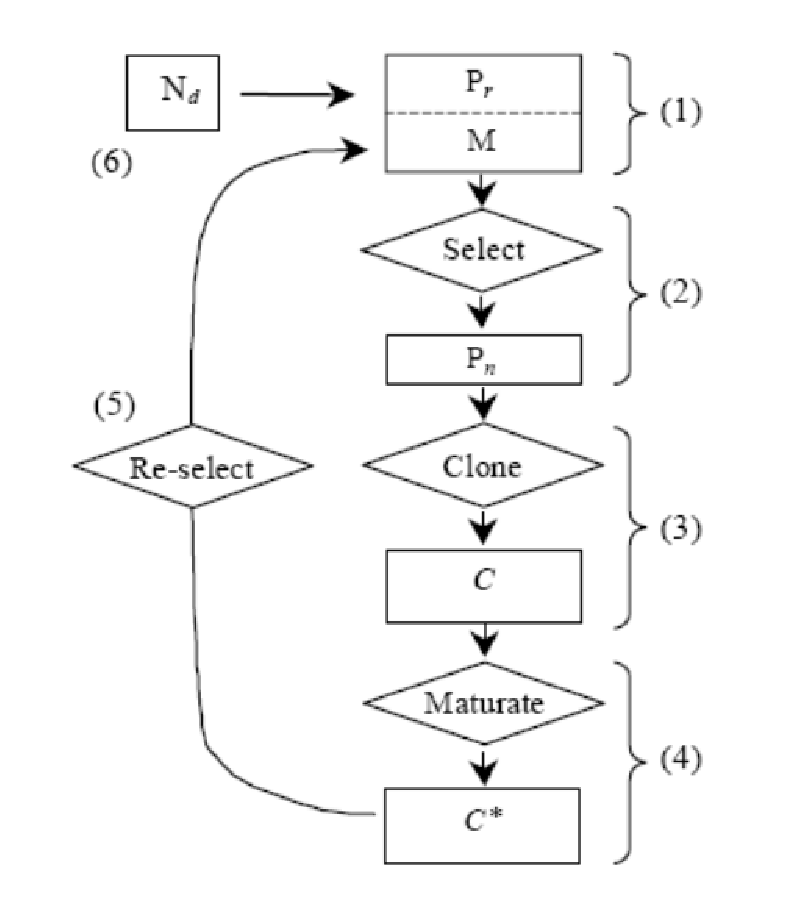
\includegraphics[width=0.5\textwidth]{img/algoritmo}
\end{center}
\caption{Diagrama del algoritmo de la selección clonal}
\label{fig:algoritmo}
\end{figure}

Siendo la explicación de los pasos de la figura~\ref{fig:algoritmo} la siguiente:
\begin{enumerate}
    \item Generar un conjunto (P) de soluciones candidatas, compuesto de células de memoria (M) añadidas a la población restante (Pr), teniendo entonces $P = Pr + M$
    \item Determinar los $n$ mejores individuos (Pn) de la población (P), basado en una medida de afinidad.
    \item Clonar (reproducir) estos $n$ mejores individuos de la población, dando origen a una población temporal de clones (C).
    \item Someter la población de clones a un esquema de hiper-mutación (proporcional a la afinidad del anticuerpo). Una población de anticuerpos maduros es generada (C*).
    \item Seleccionar nuevamente los mejores individuos de (C*) para componer el conjunto de memoria. (Algunos reemplazos desde (C*) a (P), debido a la mejora)
    \item Reemplazar los $d$ anticuerpos con menor afinidad de la población, manteniendo la diversidad.
\end{enumerate}


\label{sec:tecnica}

\subsection{Algoritmo propuesto}
\subsubsection{Componentes}
% Descripción los componentes que se probaron.
% Ej. AIS: Operadores de seleccion,
%		   Operadores de clonacion,
%		   Operadores de reemplazo,
%		   Movimientos,
%		   Funciones objetivos, etc.
% Resultados de las pruebas realizadas (tablas o gráficos). Ejemplo:
%	\begin{table}
%	\centering
%	\begin{tabular}{| l | c | c | c | c |}
%	\hline
%	 fobj & primeros & ruleta & torneo & random \\
%	\hline
%	 instancia 1 & 33000 &  31000 & 30000 & 40000 \\
%	\hline
%	 instancia 2 & 56000 &  45000 & 47000 & 60000 \\
%	\hline
%	\end{tabular}
%	\caption{Resultados pruebas Operadores de selecci\'on}
%	\end{table}
\begin{enumerate}
	\item \textbf{Operador de Selección}
		% 1. Seleccion por ruleta

		Al momento de seleccionar individuos para realizar la clonación, se utilizó la conocida técnica llamada
		\emph{roulette wheel}, para una Función Objetivo que minimiza.
		
		El procedimiento es bien simple, sólo tenemos que considerar el \emph{fitness} de cada linfocito y calcular un
		\emph{fitness relativo} de la siguiente forma:
		
		$$relativeFitness_{i}\ = \frac{f_{min} + f_{max} - f_{i}}{\sum\limits_{i=0}^{sizePop} (f_{min} + f_{max} - f_{i}}$$
		
		Donde $f_{max}$ equivale al \emph{fitness} del mejor linfocito,
		$f_{min}$ equivale al \emph{fitness} del peor linfocito y
		$f_{i}$ equivale al \emph{fitness} del i-ésimo linfocito de nuestra población.
		
		La suma de todos los \emph{fitness relativo} equivale a $1$.
			
		Luego de que cada linfocito posee su \emph{fitness relativo}, se procede a calcular un \emph{fitness acumulativo},
		es decir, ir sumando las probabilidades para generar un rango entre $0$ y $1$ con todas nuestras probabilidades.
			
		Una vez se tiene el \emph{fitness acumulativo} listo, se procede a obtener un número aleatorio entre $0$ y $1$,
		para que luego sea ubicado en nuestro rango, y así el linfocito que salga escogido con éste número aleatorio, será
		elegido para pasar ahora a la transformación.

		% 2. Seleccionar siempre los mejores
		% Pendiente

		% Tabla comparativa

	\item \textbf{Operador de Clonación}
		% 1. Clonación una cantidad aleatoria de veces
		% Pendiente


		% 2. Clonacion por fórmula
		% Pendiente
			

		% Tabla comparativa
	\item \textbf{Operador de Reemplazo}
		% 1. Reemplazo aleatorio
		% Pendiente


		% 2. Reemplazo de los más malos
		% Pendiente


		% Tabla comparativa
	\item \textbf{Movimiento}
		% 1. Swap con 10%
		% 2. Swap con 20%

		En éste caso se realiza un \emph{swap}, pero como cada individuo es del orden de $200$, $300$ y $400$ autos,
		se realiza una cantidad de \emph{swap} equivalente al $10\%$ y $20\%$ de la cantidad de autos.
	
		Para ver que elementos hacen el \emph{swap}, se eligen aleatoriamente dos elementos para intercambiar.~\footnote{
		Éste proceso se podría mejorar, estudiando a fondo que swaps nos convienen más, para obtener siempre mejores
		resultados}


		% Tabla comparativa
\end{enumerate}

\label{sec:componentes}

\subsubsection{Algoritmo Final}
% Pseudo codigo del algoritmo final
%  (con los componentes elegidos a traves de las pruebas y su criterio).
% En lo posible adjuntar una tabla de los resultados encontrados por
%  su algoritmo y otros algoritmos de la literatura
%  (no es importante que sean buenos, es solo para comparar en que punto se encuentra). 

\label{sec:algoritmo}

\newpage
\section{Bibliografía}
\bibliography{informe2}
\newpage

\section{Anexo}
\subsection{Promedio}

\begin{figure}[H]
\begin{center}
\includegraphics[width=0.95\textwidth]{img/prom-1.pdf}
\end{center}
\caption{Promedio de valores para cada modificación}
\label{fig:prom-1}
\end{figure}

\begin{figure}[H]
\begin{center}
\includegraphics[width=0.95\textwidth]{img/prom-2.pdf}
\end{center}
\caption{Promedio de valores para cada modificación}
\label{fig:prom-2}
\end{figure}

\begin{figure}[H]
\begin{center}
\includegraphics[width=0.95\textwidth]{img/prom-3.pdf}
\end{center}
\caption{Promedio de valores para cada modificación}
\label{fig:prom-3}
\end{figure}


\begin{figure}[H]
\begin{center}
\includegraphics[width=0.95\textwidth]{img/prom-4.pdf}
\end{center}
\caption{Promedio de valores para cada modificación}
\label{fig:prom-4}
\end{figure}

\newpage

\subsection{Desviación estándar}

\begin{figure}[H]
\begin{center}
\includegraphics[width=0.95\textwidth]{img/s-1.pdf}
\end{center}
\caption{Desviación estándar para cada modificación.}
\label{fig:s-1}
\end{figure}

\begin{figure}[H]
\begin{center}
\includegraphics[width=0.95\textwidth]{img/s-2.pdf}
\end{center}
\caption{Desviación estándar para cada modificación.}
\label{fig:s-2}
\end{figure}

\begin{figure}[H]
\begin{center}
\includegraphics[width=0.95\textwidth]{img/s-3.pdf}
\end{center}
\caption{Desviación estándar para cada modificación.}
\label{fig:s-3}
\end{figure}

\begin{figure}[H]
\begin{center}
\includegraphics[width=0.95\textwidth]{img/s-4.pdf}
\end{center}
\caption{Desviación estándar para cada modificación.}
\label{fig:s-4}
\end{figure}

\newpage

\subsection{Valores máximos}

\begin{figure}[H]
\begin{center}
\includegraphics[width=0.95\textwidth]{img/max-1.pdf}
\end{center}
\caption{Valores máximos para cada modificación}
\label{fig:max-1}
\end{figure}

\begin{figure}[H]
\begin{center}
\includegraphics[width=0.95\textwidth]{img/max-2.pdf}
\end{center}
\caption{Valores máximos para cada modificación}
\label{fig:max-2}
\end{figure}

\begin{figure}[H]
\begin{center}
\includegraphics[width=0.95\textwidth]{img/max-3.pdf}
\end{center}
\caption{Valores máximos para cada modificación}
\label{fig:max-3}
\end{figure}

\begin{figure}[H]
\begin{center}
\includegraphics[width=0.95\textwidth]{img/max-4.pdf}
\end{center}
\caption{Valores máximos para cada modificación}
\label{fig:max-4}
\end{figure}


\newpage

\subsection{Valores mínimos}

\begin{figure}[H]
\begin{center}
\includegraphics[width=0.8\textwidth]{img/min-1.pdf}
\end{center}
\caption{Valores mínimos para cada modificación}
\label{fig:min-1}
\end{figure}

\begin{figure}[H]
\begin{center}
\includegraphics[width=0.8\textwidth]{img/min-2.pdf}
\end{center}
\caption{Valores mínimos para cada modificación}
\label{fig:min-2}
\end{figure}

\begin{figure}[H]
\begin{center}
\includegraphics[width=0.8\textwidth]{img/min-3.pdf}
\end{center}
\caption{Valores mínimos para cada modificación}
\label{fig:min-3}
\end{figure}

\begin{figure}[H]
\begin{center}
\includegraphics[width=0.8\textwidth]{img/min-4.pdf}
\end{center}
\caption{Valores mínimos para cada modificación}
\label{fig:min-4}
\end{figure}


\newpage
\subsection{Tiempo de ejecución}

\begin{figure}[H]
\begin{center}
\includegraphics[width=0.95\textwidth]{img/t-1.pdf}
\end{center}
\caption{Tiempo de ejecución para las modificaciones en cada instancia}
\label{fig:t-1}
\end{figure}

\begin{figure}[H]
\begin{center}
\includegraphics[width=0.95\textwidth]{img/t-2.pdf}
\end{center}
\caption{Tiempo de ejecución para las modificaciones en cada instancia}
\label{fig:t-2}
\end{figure}

\begin{figure}[H]
\begin{center}
\includegraphics[width=0.95\textwidth]{img/t-3.pdf}
\end{center}
\caption{Tiempo de ejecución para las modificaciones en cada instancia}
\label{fig:t-3}
\end{figure}

\begin{figure}[H]
\begin{center}
\includegraphics[width=0.95\textwidth]{img/t-4.pdf}
\end{center}
\caption{Tiempo de ejecución para las modificaciones en cada instancia}
\label{fig:t-4}
\end{figure}

\label{sec:anexo}

\end{document} 
